\chapter{Communication Systems : Part - I}\label{chap9}

Communication is a vital component in a progressive world. It enhances people's lives to great extent. Satellite television, fax machine and cellular phones are some examples of communication systems. This chapter discusses basics of communication, various types of modulation and demodulation.

\section{Communication}\label{sec9.1}

Communication is the process of transfering information meaningfully from one point to another. In general, electronic communication refers to the sending, receiving and processing of information by electronic means. Meaningful information may be in the form of voice, text, picture or a combination of these.

A modern communication system involves the following stages. 
\begin{enumerate}
\item Sorting, processing and storing of information prior to communication.

\item Transmission with further processing and filtering of noise or unwanted information.

\item Reception of information, which includes processing steps to obtain an estimate or interpretation of the message or information.
\end{enumerate}

\section{Elements of communication systems}\label{sec9.2}
\index{Communication systems!elements of}

A communication system\index{Communication systems} is an integration of various equipment needed for the process of communication. Fig.~\ref{fig9.1} shows the block diagram of a general communication system. The function of each block is explained below.

\heading{\em Information source:}
The main aim of a communication system is to convey a message called information. This message originates from an information source.
\begin{figure}[H]
\centering
\includegraphics{chap9/S3-EE-07-002.eps}
\caption{Block diagram of a communication system}\label{fig9.1}
\end{figure}

\smallskip
\heading{\em Transmitter:}\index{Transmitter}
It processes the input message signal to make it suitable for sending it over the channel. This operation termed as modulation, which is a process that changes or modulates the characteristics of a high frequency signal called the carrier in accordance with the message signal.

\smallskip
\heading{\em Channel:}\index{Channel}
It is the physical medium or path that connects the transmitter and receiver. This may be a pair of wires such as telephone wires or free space. The term {\em channel} is often used to refer to the frequency range allocated to a particular service or transmission such as a television channel.

\smallskip
\heading{\em Noise:}\index{Noise}
Noise is an unwanted signal that gets added to the message signal during transmission over the channel. It is random in nature and has its greatest effect when the message signal is weakest.

\smallskip
\heading{\em Receiver:}\index{Receiver}
The receiver processes the signal and makes an estimate of the actual message that is transmitted. It performs a process called demodulation, which is the reverse of modulation and extracts the information superimposed on the carrier wave. The receiver, in addition to demodulation also performs amplification and filtering. 

\section{Modulation}\label{sec9.3}
\index{Modulation}

In a communication system, the transmitter modifies the message signal into a form suitable for transmission over the channel, by using a process known as modulation.

Modulation is defined as the process by which some characteristic or property of a high frequency sine wave called the carrier is varied in accordance with the instantaneous amplitude of the message signal called the modulating signal.

\vskip .1cm

A sine wave carrier which is a high frequency signal, may be represented by the equation
\begin{equation}
v_{c}=V_{c}\sin (\omega_{c}t+\phi)\label{eq9.1}
\end{equation}
where
\vskip -1.3cm
\begin{align*}
v_{c} &= \text{the instantaneous value of the carrier}\\
V_{c} &= \text{the peak or maximum amplitude of the carrier}\\
\omega_{c} &= \text{the angular frequency of the carrier}\\
\phi &= \text{the phase angle of the carrier with respect to some reference}
\end{align*}

The characteristic of the carrier wave that is modified may be amplitude, frequency or phase angle. Accordingly, we have three types of modulation, namely,
\begin{enumerate}
\itemsep=0pt
\item Amplitude modulation

\item Frequency modulation

\item Phase modulation
\end{enumerate}

\section{Classification of communication systems based on the modulation scheme and input signal}\label{sec9.4}
\index{Communication systems!classification of}

Based on the modulation scheme and input signal, communication systems may be classified as follows:
\begin{enumerate}
\itemsep=0pt
\item {\em Analog communication system:} This transmits analog input signals using analog modulation schemes.

\item {\em Digital communication system:} This transmits digital information using digital modulation schemes.

\item {\em Hybrid communication system:} This converts analog input signal into digital format and transmits it using digital modulation techniques.
\end{enumerate}

\section{Need for modulation in communication systems}\label{sec9.5}
\index{Modulation!need for}

Modulation is needed for the following reasons:

\smallskip
\heading{1. Long distance communication}
\index{Long distance communication}

Most of the message signals are low audio frequency signals lying within the range of 20Hz to 20kHz. Direct transmission without modulation, of such low frequency signals over long distances would require enormous power. With modulation the frequency of the signal to be transmitted is increased and consequently signals can be transmitted over long distances with considerably lower in power.

\smallskip
\heading{2. Practical size of antenna}

Transmission of signals in the form of electromagnetic waves cannot be done without the use of antennas. For efficient transmission and reception the heights of the transmitting and receiving antennas should be comparable to quarter-wavelength of the frequency of the signal used. This is 75 meters at 1 MHz, but increases to 5000 meters or 16000 feet at 15 kHz. A vertical antenna of this height is unimaginable. Since modulation uses a high frequency carrier for transmission the height of antennas is considerably reduced to practical values.

\smallskip
\heading{3. Avoid mixing of audio signals}

When a number of stations transmit sound or audio signals directly, the signals get mixed up as all of them fall within the range from 20Hz to 20kHz. Consequently, proper reception of the signals at the receiver would be very difficult. With modulation, each station is allotted a different carrier frequency and the signal from a station can be properly received by tuning the receiver to that particular carrier frequency.\\[-20pt]

\section{Frequency ranges and their application}\label{sec9.6}
\index{Frequency ranges}

Table~\ref{tab9.1} lists the frequency ranges and their applications.
\begin{table}[H]
\centering
\caption{Frequency ranges and their usage}\label{tab9.1}
\renewcommand{\arraystretch}{1.15}
{\fontsize{10pt}{12pt}\selectfont
\begin{tabular}{|lcl|}
\hline
\multicolumn{1}{|c}{\it\bfseries Frequency range} & & \multicolumn{1}{c|}{\it\bfseries Application}\\
\hline
Super high frequencies 3 GHz-30 GHz & $\to$ & Radar\\
\hline
Ultra high frequencies 300 MHz-3 GHz & $\to$ & Communication satellites, cellular phones,\\[-4pt]
 & & personal communication systems\\
\hline
Very high frequencies 30 MHz-300 MHz & $\to$ & TV and FM broadcast\\
\hline
High frequencies 3 MHz-30 MHz & $\to$ & Short-wave broadcast commercial\\
\hline
Medium frequencies 300 kHz-3 MHz & $\to$ & AM broadcast\\
\hline
Low frequencies 30 kHz-300 kHz & $\to$ & Navigation, submarine communications\\
\hline
Very low frequencies 3 kHz-30 kHz & $\to$ & Submarine communications, navigation\\
\hline
Voice frequencies 300 Hz-3 kHz & $\to$ & Audio, submarine communication, navigation\\
\hline
Extremely low frequencies 30 Hz-300 Hz & $\to$ & Power transmission\\
\hline
\end{tabular}}\relax
\end{table}

The velocity $(v)$, frequency $(f)$ \ and wavelength $(\lambda)$ of a wave are related by
\begin{align}
v &= f\lambda\label{eq9.2}\\[3pt]
\lambda &= \frac{v}{f}\label{eq9.3}
\end{align}

Note that, the wavelength of the wave is inversely proportional to the frequency of the wave. The following terminologies are commonly used in communication.
\begin{quote}
Long wave~: low frequency signal.

Short wave~: High frequency signal.

Microwave~: Signal with frequency in gigahertz range.\\[-20pt]
\end{quote}

\section{Amplitude modulation}\label{sec9.7}
\index{Amplitude modulation}\index{Modulation!amplitude modulation}

Amplitude modulation or AM is defined as a process in which the amplitude of the high frequency sinusoidal carrier wave is made to vary in accordance with the instantaneous amplitude of the low frequency message signal called modulating signal.

The frequency and phase angle of the carrier are unaffected in amplitude modulation.

Let $v_{c}$ and $v_{m}$ represent the instantaneous values of the carrier voltage and modulating voltage given respectively by
\begin{equation}
v_{c}=V_{c}\sin \omega_{c}t\label{eq9.4}
\end{equation}
and
\begin{equation}
v_{m}=V_{m}\sin \omega_{m}t\label{eq9.5}
\end{equation}
where,
\vskip -1cm
\begin{align*}
V_{c} &= \text{Peak amplitude of the unmodulated carrier wave}\\[3pt]
V_{m} &=\text{Peak amplitude of modulating signal}
\end{align*}

In the above expressions, the phase angle has been omitted as it is unaffected by amplitude modulation.

After amplitude modulation, the peak amplitude of the carrier wave is proportional to $v_{m}$ and is given by
\begin{equation}
A(t)=V_{c}+Kv_{m}\label{eq9.6}
\end{equation}
where, $K$ is the proportionality constant, known as the amplitude sensitivity of modulation, which is usually made equal to unity
\begin{equation}
\therefore\quad A(t)=V_{c}+v_{m}\label{eq9.7}
\end{equation}

The principle of amplitude modulation is illustrated in Fig.~\ref{fig9.2} which shows a single frequency sinusoidal voltage modulating a high frequency carrier signal.

Fig.~\ref{fig9.2} shows amplitude modulated wave for one cycle of the modulating sine wave. When there is no modulation, the amplitude of the carrier is equal to its unmodulated value $V_{c}$. When modulation is present the amplitude of the carrier is varied by the instantaneous value of the modulating sine wave and is given by
\begin{equation}
A(t)=V_{c}+v_{m}=V_{c}+V_{m}\sin \omega_{m}t\label{eq9.8}
\end{equation}
\begin{figure}[H]
\centering
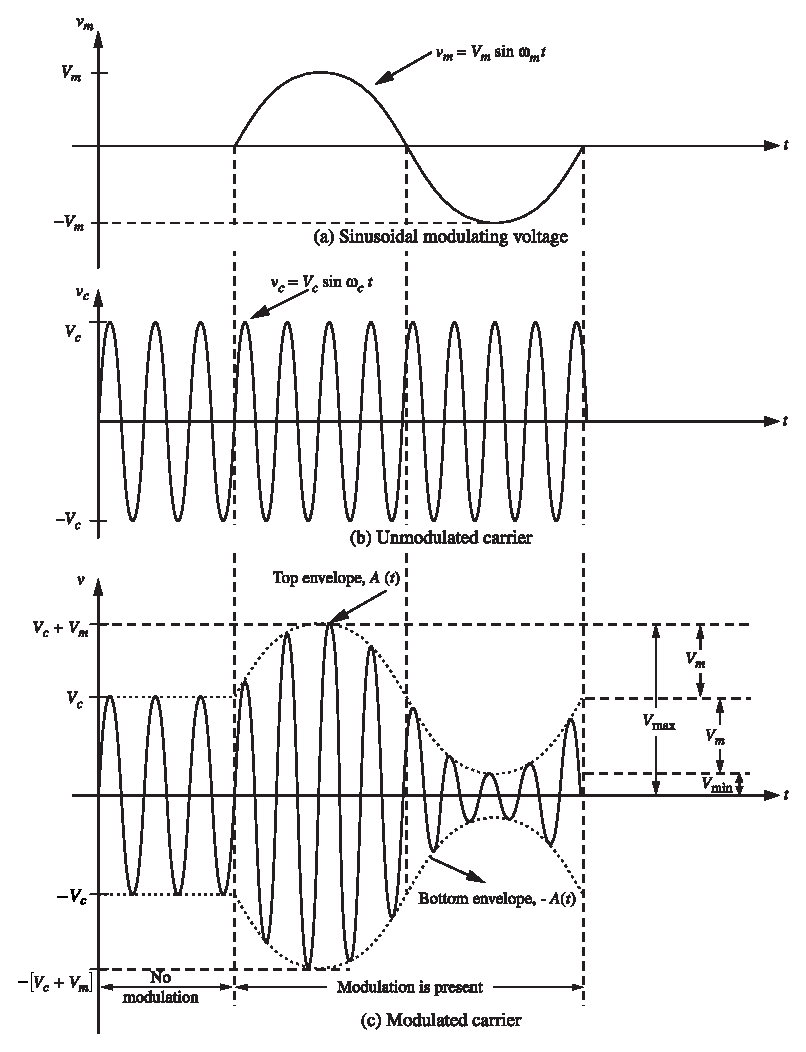
\includegraphics[scale=1.05]{chap9/S3-EE-07-003.eps}
\caption{Amplitude modulation}\label{fig9.2}
\end{figure}

\section{Modulation index of amplitude modulation}\label{sec9.8}
\index{Amplitude modulation!modulation index}

Fig.~\ref{fig9.3} shows that distortion will occur if the value of $V_{m}$ exceeds that of $V_{c}$. Hence, the amplitude of modulating voltage, $V_{m}$ must be less than the amplitude of the carrier, $V_{c}$ for proper and undistorted amplitude modulation. The relationship between $V_{m}$ and $V_{c}$ called modulation index or depth of modulation $m_{a}$, is defined as the ratio of the amplitude of the modulating voltage to the amplitude of the carrier wave and is given by
\begin{equation}
m_{a}=\frac{V_{m}}{V_{c}}\label{eq9.9}
\end{equation}
\vskip -.3cm
\begin{figure}[H]
\centering
\includegraphics[scale=.9]{chap9/S3-EE-07-004.eps}
\smallskip
\caption{Amplitude of AM wave}\label{fig9.3}
\end{figure}

Modulation index\index{Modulation index} is a number that lies between 0 and 1 for distortion less modulation and is usually expressed as a percentage, called the percentage modulation, given by,
\begin{equation}
\text{\%~} \ m_{a}=\frac{V_{m}}{V_{c}}\times 100\text{\%}\label{eq9.10}
\end{equation}

\section{Expression for the instantaneous voltage of amplitude modulated wave : AM wave equation}\label{sec9.9}
\index{Amplitude modulation!wave equation}

Consider the amplitude modulation in which the modulating voltage is given by
\begin{equation}
v_{m}=V_{m}\sin \omega_{m}t\label{eq9.11}
\end{equation}
and the carrier voltage is given by
\begin{equation}
v_{c}=V_{c}\sin \omega_{c}t\label{eq9.12}
\end{equation}

Since amplitude modulation varies the amplitude of the carrier in accordance with the instantaneous value of the modulating voltage, $v_{m}$, the amplitude of the modulated carrier or AM wave is given by
\begin{equation}
A(t)=V_{c}+v_{m}=V_{c}+V_{m}\sin \omega_{m}t\label{eq9.13}
\end{equation}

The instantaneous voltage of the amplitude modulated wave is, therefore
\begin{align*}
v &= A(t)\sin \omega_{c}t\\[2pt] 
 &= (V_{c}+V_{m}\sin \omega_{m}t)\sin \omega_{c}t\\[2pt]
  &= V_{c}\left(1+\frac{V_{m}}{V_{c}}\sin \omega_{m}t\right)\sin \omega_{c}t
\end{align*}
\indent
From Eqn.~\eqref{eq9.9},
\begin{align}
\frac{V_{m}}{V_{c}} &= m_{a}\notag\\[2pt]
\therefore\quad v &= V_{c}\,(1+m_{a}\sin \omega_{m}t)\sin \omega_{c}t\label{eq9.14}\\[2pt]
v &= V_{c}\sin \omega_{c}t+V_{c}\,m_{a}\sin \omega_{c}t\sin \omega_{m}t\label{eq9.15}
\end{align}
using the trigonometric relation
\begin{align}
\sin A\sin B &= \frac{1}{2}[\cos (A-B)-\cos(A+B)],\quad\text{we get}\notag\\[2pt]
v &= V_{c}\sin \omega_{c}t +\frac{m_{a}V_{c}}{2}\cos (\omega_{c}-\omega_{m})t-\frac{m_{a}V_{c}}{2}\cos (\omega_{c}+\omega_{m})t\label{eq9.16}
\end{align}
This is the expression for the instantaneous voltage of amplitude modulated wave.

\section{Expression for modulation index of amplitude modulation}\label{sec9.10}
\index{Amplitude modulation!modulation index of}

An expression for modulation index can be obtained in terms of the maximum and minimum amplitudes, $V_{\max}$ and $V_{\min}$ of the amplitude modulated wave shown in Fig.~\ref{fig9.2}(c). From Fig.~\ref{fig9.2}(c) we have
\begin{align}
2V_{m}+V_{\min} &= V_{\max}\notag\\[4pt]
\therefore\quad V_{m} &= \frac{V_{\max}-V_{\min}}{2}\label{eq9.17}
\end{align}
where, $V_{m}=$ amplitude of modulating voltage, and from Fig.~\ref{fig9.2}(c)
\begin{equation}
V_{c}=V_{m}+V_{\min}\label{eq9.18}
\end{equation}
where, $V_{c}=$ amplitude of unmodulated carrier.

Substituting for $V_{m}$ from Eqn.~\eqref{eq9.17} into Eqn.~\eqref{eq9.18}. We get
\begin{align}
V_{c} &= \frac{V_{\max}-V_{\min}}{2}+V_{\min}\qquad
\text{or}\qquad V_{c} = \frac{V_{\max}+V_{\min}}{2}\label{eq9.19}
\end{align}

Dividing Eqn.~\eqref{eq9.17} by Eqn.~\eqref{eq9.19} we get the expression for modulation index $m_{a}$ as
\begin{align}
m_{a} &= \frac{V_{m}}{V_{c}}=\frac{(V_{\max}-V_{\min})/2}{(V_{\max}+V_{\min})/2}
= \frac{V_{\max}-V_{\min}}{V_{\max}+V_{\min}}\label{eq9.20}
\end{align}
Eqn.~\eqref{eq9.20} is the standard procedure to calculate the modulation index of AM wave, by observing on an oscilloscope.

\subsection{Effect of modulation index on amplitude modulation}\label{sec9.10.1}

The extent to which the amplitude of the carrier is varied in amplitude modulation depends on the value of the modulation index, $m_{a}$. Based on the value of modulation index, we have the three cases of modulation:
\begin{enumerate}
\itemsep=0pt
\item $m_{a}>1$: In this case $V_{m}>V_{c}$, the carrier is said to be over damped and the AM wave or envelope is distorted due to over modulation.

\item $m_{a}<1$: In this case $V_{m}<V_{c}$, and the carrier is said to be under-damped.

\item $m_{a}=1$: In this case $V_{m}=V_{c}$, and the carrier is said to be critically or level-damped.
\end{enumerate}
These three cases are illustrated in Fig.~\ref{fig9.4}.\\[-20pt]

\subsection{Significance of modulation index}\label{sec9.10.2}

In an AM wave the signal or information is contained in the variation of the carrier amplitude. The degree of modulation or modulation index is an indication of the strength of the message signal i.e., the greater the modulation index, $m_{a}$, the stronger and clearer will be the message signal. Thus, for $m_{a}=1$ or $100\%$, the message signal being transmitted will be the strongest. However, when the carrier is over modulated i.e., for $m_{a}>1$ or $100\%$ the AM wave will be clipped off and a large distortion will occur during reception. Hence modulation index should never exceed 1 or 100\%.\\[-20pt]

\subsection{Frequency spectrum of AM wave and its bandwidth}\label{sec9.10.3}
\index{Amplitude modulation!frequency spectrum of}

Frequency spectrum is a plot of amplitude versus frequency of a wave.

Eqn.~\eqref{eq9.16} shows that the AM wave contains three terms. 
\begin{itemize}
\itemsep=0pt
\item[$\bullet$] The first term, $V_{c}\sin \omega_{c}t$ represents the unmodulated carrer of frequency, $f_{c}$.

\item[$\bullet$] The second term, $\dfrac{m_{a}V_{c}}{2}\cos (\omega_{c}-\omega_{m})t$ represents the lower sideband of frequency,
\begin{equation}
f_{LSB}=f_{c}-f_{m}\label{eq9.21}
\end{equation}

\item[$\bullet$] The third term, $\dfrac{m_{a}V_{c}}{2}\cos (\omega_{c}+\omega_{m})t$ represents the upper side band of frequency,
\begin{equation}
f_{USB}=f_{c}+f_{m}\label{add-eq9.22}
\end{equation}
\end{itemize}

\vfill\eject

\begin{figure}[H]
\centering
\includegraphics[scale=.91]{chap9/S3-EE-07-005abc.eps}
\caption{Effect of modulation index on Amplitude modulation}\label{fig9.4}
\end{figure}

The amplitude of the two sidebands are the same and equal to $\dfrac{m_{a}V_{c}}{2}$. Fig.~\ref{fig9.5} shows the plot of the frequency spectrum of the amplitude modulated wave.
\begin{figure}[H]
\centering
\includegraphics{chap9/S3-EE-07-006.eps}
\caption{Frequency spectrum of AM wave}\label{fig9.5}
\end{figure}

In practice, the carrier frequency $f_{c}$ is very much greater than the modulating frequency $f_{m}$ and hence the sideband frequencies are very close to the carrier frequency. Also, the AM wave is a voltage or a current wave.

In case of AM wave the bandwidth is the difference between the sideband frequencies.
\begin{equation}
BW=f_{\text{USB}}-f_{\text{LSB}}=(f_{c}+f_{m})-(f_{c}-f_{m})=2f_{m}\label{eq9.23}
\end{equation}
Thus, the bandwidth of amplitude modulation is twice the signal or modulating frequency.

\begin{example}\label{exam9.1}
An audio signal of $1$ kHz is used to amplitude modulate a carrier of $600$ kHz. Determine (a) side band frequencies and (b) bandwidth required.
\end{example}

\begin{solution}
Given~ $f_{c}=600$\,kHz and $f_{m}=1$\,kHz.

The sideband frequencies are
$$
f_{\text{LSB}}=f_{c}-f_{m}=600\text{kHz}-1\text{kHz}=599\text{~kHz}
$$
and
$$
f_{\text{USB}}=f_{c}+f_{m}=600\text{kHz}+1\text{kHz}=601\text{~kHz}
$$

The bandwidth required is
$$
BW=2f_{m}=2\times 1\text{kHz}=2\text{\,kHz}
$$
\vskip -.7cm
\end{solution}

\eject

\section{Expression for the total average power of a sinusoidal AM wave}\label{sec9.11}
\index{Amplitude modulation!power of}

The instantaneous value of an AM wave is given by Eqn.~\eqref{eq9.16} as
$$
v=V_{c}\sin \omega_{c}t+\dfrac{m_{a}V_{c}}{2}\cos (\omega_{c}-\omega_{m})t-\dfrac{m_{a}V_{c}}{2}\cos (\omega_{c}+\omega_{m})t
$$
which shows that AM wave has three components namely, the unmodulated carrier, the lower sideband and the upper sideband. Hence, the total power $P_{t}$ transmitted by amplitude modulated wave is the sum of the carrier power $P_{c}$ and the power in the two sidebands, $P_{\text{LSB}}$ and $P_{\text{USB}}$.

Thus,
\begin{align*}
P_{t} &= P_{c}+P_{\text{LSB}}+P_{\text{USB}}
\end{align*}

We know that the average power is given by
\begin{align}
\text{Power} &= \frac{\text{(rms Voltage)}^{2}}{\text{resistance}}\notag\\[3pt]
\therefore\quad P_{t} &= \frac{V^{2}_{\carr}}{R}+\frac{V^{2}_{\text{LSB}}}{R}+\frac{V^{2}_{\text{USB}}}{R}\label{eq9.24}
\end{align}

Where,
\begin{align*}
P_{t} &= \text{total average power delivered}\\[4pt]
V_{\carr} &= \text{rms value of the unmodulated carrier}\\[4pt]
V_{\text{LSB}} &= \text{rms value of the lower sideband}\\[4pt]
V_{\text{USB}} &= \text{rms value of the upper sideband}\\[4pt]
R &= \text{resistance of the transmitting antenna in which power is dissipated}
\end{align*}

Since, the carrier and sidebands are sinusoidal voltages
\begin{equation}
V_{\carr} =\frac{V_{c}}{\sqrt{2}}\label{eq9.25}
\end{equation}
and
\begin{equation}
V_{\text{LSB}}=V_{\text{USB}}=\frac{(m_{a}V_{c}/2)}{\sqrt{2}}\label{eq9.26}
\end{equation}

Using Eqn.~\eqref{eq9.25}, the power in the unmodulated carrier is given by
\begin{equation}
P_{c} = \frac{(V_{c}/\sqrt{2})^{2}}{R}=\frac{V^{2}_{c}}{2R}\label{eq9.27}
\end{equation}

Using Eqn.~\eqref{eq9.26}, the power in the sidebands is given by
\begin{equation}
P_{\text{LSB}}=P_{\text{USB}}=\frac{1}{R}\left(\frac{m_{a}V_{c}/2}{\sqrt{2}}\right)^{2}=\dfrac{m^{2}_{a}}{4}\frac{V^{2}_{c}}{2R}=\frac{m^{2}_{a}}{4}P_{c}\label{eq9.28}
\end{equation}

Thus the total power in the amplitude modulated wave is
\begin{equation}
P_{t}=\frac{V^{2}_{c}}{2R}+\frac{m^{2}_{a}}{4}\frac{V^{2}_{c}}{2R}+\frac{m^{2}_{a}}{4}\frac{V^{2}_{c}}{2R}\label{eq9.29}
\end{equation}
since $\dfrac{V^{2}_{c}}{2R}=P_{c}$, the above equation can be written as
$$
P_{t}=P_{c}+\frac{m^{2}_{a}}{4}P_{c}+\frac{m^{2}_{a}}{4}P_{c}
$$
or
\begin{equation}
P_{t}=P_{c}\left(1+\dfrac{m^{2}_{a}}{2}\right)\label{eq9.30}
\end{equation}

Eqn.~\eqref{eq9.30} shows that the total power in the amplitude modulated wave is
\begin{itemize}
\item more than that of unmodulated carrier.

\item dependent on the modulation index $m_{a}$.
\end{itemize}

\begin{example}\label{exam9.2}
A $400$W carrier is modulated to a depth of 75\%. Calculate the total power in the modulated wave.
\end{example}

\begin{solution}
Given $P_{c}=400$\,W, $m_{a}=75\%=0.75$.

The total power is
$$
P_{t}=(400\,\text{W})\left(1+\dfrac{0.75^{2}}{2}\right)=512.5\text{W}
$$
\vskip -.7cm
\end{solution}

\begin{example}
A local AM transmitter broadcasts a carrier power of $50$\,kW. Determine the radiated power at a modulation index of 0.6.
\end{example}

\begin{solution}
Given $P_{c}=50$\,kW, $m_{a}=0.6$.
$$
P_{t}=P_{c}\left(1+\dfrac{m^{2}_{a}}{2}\right)=(50\,\text{kW})\left(1+\dfrac{0.6^{2}}{2}\right)=59\text{\;kW}
$$
\vskip -.7cm
\end{solution}

\eject

\section{Maximum power in an AM wave}\label{sec9.12}
\index{Amplitude modulation!maximum power in}

From Eqn.~\eqref{eq9.30} the total power in the AM wave is
$$
P_{t}=P_{c}\left(1+\dfrac{m^{2}_{a}}{2}\right)
$$

It is easy to see that $P_{t}$ is maximum when $m_{a}$ is maximum.

The maximum value of $m_{a}=1$, at which
\begin{equation}
P_{t}=P_{c}\left(1+\dfrac{1}{2}\right)=1.5P_{c}\label{eq9.31}
\end{equation}
Thus the maximum power in the AM wave is $1.5P_{c}$ or $150\%$ of the carrier power $P_{c}$.

\section{Transmission efficiency of AM wave}\label{sec9.13}

The transmission efficiency of\index{Amplitude modulation!transmission efficiency of} AM wave is defined as
$$
\text{Transmission efficiency,~ } \eta= \dfrac{\text{transmitted power that contains information}}{\text{total transmitted power, $P_{t}$}}
$$

Since, the transmitted power that contains the information is the sideband power,\break $P_{\text{SB}}=P_{\text{LSB}}+P_{\text{USB}}$, we have
\begin{equation}
\eta = \frac{P_{\text{LSB}}+P_{\text{USB}}}{P_{t}}\label{eq9.32}
\end{equation}

From Eqn.~\eqref{eq9.28},
\begin{equation}
P_{\text{LSB}}=P_{\text{USB}}=\frac{m^{2}_{a}}{4}\frac{V^{2}_{c}}{2R}=\frac{m^{2}_{a}}{4}P_{c}\label{eq9.33}
\end{equation}

Substituting Eqns.~\eqref{eq9.30} and \eqref{eq9.33} into Eqn.~\eqref{eq9.32} we get
$$
\eta = \frac{\frac{m^{2}_{a}}{4}P_{c}+\frac{m^{2}_{a}}{4}P_{c}}{P_{c}\left(1+\frac{m^{2}_{a}}{2}\right)}=\dfrac{\frac{m^{2}_{a}}{2}}{1+\frac{m^{2}_{a}}{2}}
$$
or
\begin{equation}
\eta=\dfrac{m^{2}_{a}}{2+m^{2}_{a}}\label{eq9.34}
\end{equation}

The percentage transmission efficiency is
\begin{align}
\%\ \eta &= \frac{m^{2}_{a}}{2+m^{2}_{a}}\times 100\%\notag\\[3pt]
\text{or}\quad \% \ \eta &= \frac{m^{2}_{a}}{m^{2}_{a}\left(1+\frac{2}{m^{2}_{a}}\right)}=\dfrac{1}{1+\dfrac{2}{m^{2}_{a}}}\label{eq9.35}
\end{align}

This shows that the transmission efficiency increases with modulation index. This happens as the sideband power $P_{\text{SB}}$, which corresponds to the information power, increases with increase in modulation index.

\smallskip
\noindent
\underline{\bf When~ \boldmath$m_{a}=1$~ or~ $100\%$}
$$
\% \ \eta =\dfrac{1^{2}}{2+1^{2}}\times 100\% = 33.3\%
$$

Hence the maximum transmission efficiency of the AM wave is 33.3\%.

\smallskip
\noindent
\underline{\bf When \boldmath$m_{a}=0.8$~ or~ $80\%$.}
$$
\% \ \eta =\dfrac{0.8^{2}}{2+0.8^{2}}\times 100 = 24.24\%
$$
Thus higher the modulation index, higher is the transmission efficiency.

\section{Modulation index in terms of carrier power and total power of the AM wave}\label{sec9.14}
\index{Amplitude modulation!modulation index}

From Eqn.~\eqref{eq9.30} the total power in the AM wave is
\begin{align}
P_{t} &= P_{c}\left(1+\dfrac{m^{2}_{a}}{2}\right)\notag\\[3pt]
\therefore\qquad \frac{P_{t}}{P_{c}} &= 1+\frac{m^{2}_{a}}{2}\notag\\[3pt]
\text{or}\qquad \frac{m^{2}_{a}}{2} &= \frac{P_{t}}{P_{c}}-1\notag\\[3pt]
\text{i.e.,}\qquad m^{2}_{a} &= 2\left(\dfrac{P_{t}}{P_{c}}-1\right)\notag\\[3pt]
\therefore\qquad m_{a} &= \sqrt{2\left(\dfrac{P_{t}}{P_{c}}-1\right)}\label{eq9.36} 
\end{align}
This is the equation for modulation index $m_{a}$ in terms of the total power, $P_{t}$ and carrier power, $P_{c}$.

\section{Modulation index and total power when a carrier is amplitude modulated by several sine waves}\label{sec9.15}

In practice, modulation of a carrier by several sine waves is very common. If $V_{1}$, $V_{2}$, $V_{3}$ etc., are the amplitudes of simultaneous sinusoidal modulating voltages, then the total modulating voltage $V_{t}$ is given by
\begin{equation}
V_{t}=\sqrt{V^{2}_{1}+V^{2}_{2}+V^{2}_{3}+\cdots}\label{eq9.37}
\end{equation}

Dividing both sides of Eqn.~\eqref{eq9.37} by $V_{c}$, the amplitude of the carrier, we get
\begin{align*}
\frac{V_{t}}{V_{c}} &= \frac{\sqrt{V^{2}_{1}+V^{2}_{2}+V^{2}_{3}+\cdots}}{V_{c}}\\[3pt]
&= \sqrt{\left(\frac{V_{1}}{V_{c}}\right)^{2}+\left(\dfrac{V_{2}}{V_{c}}\right)^{2}+\left(\frac{V_{3}}{V_{c}}\right)^{2}+\cdots}
\end{align*}

But \ $\dfrac{V_{t}}{V_{c}}=$ the total modulation index, $m_{\text{at}}$
$$
\therefore\quad m_{\text{at}}=\sqrt{m^{2}_{a1}+m^{2}_{a2}+m^{2}_{a3}+\cdots}
$$
where
$$
m_{a1}=\dfrac{V_{1}}{V_{c}},\quad m_{a2}=\dfrac{V_{2}}{V_{c}},\quad m_{a3}=\dfrac{V_{3}}{V_{c}},\quad\text{etc.,}
$$
are the individual modulation indices.

Hence, the total modulation index in modulation by several sine waves is the square root of the sum of the squares of the individual modulation indices. This total modulation index should not exceed 1.

The total power in the AM wave of the above case is given by
\begin{equation}
P_{t}=P_{c}\left(1+\frac{m^{2}_{\text{at}}}{2}\right)\label{eq9.38}
\end{equation}

\begin{example}\label{exam9.4}
A radio transmitter radiates 10\,kW when the modulation percentage is 60. Calculate the carrier power.
\end{example}

\begin{solution}
Given
\begin{align*}
P_{t} &=10\,kW,\quad m_{a}=60\% = 0.6\\[3pt]
P_{c} &= \dfrac{P_{t}}{1+\frac{m^{2}_{a}}{2}}=\frac{10\,\text{kW}}{1+\frac{0.6^{2}}{2}}=8.47\text{\,kW}
\end{align*}
\vskip -.7cm
\end{solution}

\vfill\eject

\begin{example}\label{exam9.5}
The total power content of an AM wave is $2.64\text{\,kW}$ at a modulation factor of $80\%$. Determine the power content of (i) carrier (ii) each sideband.
\end{example}

\begin{solution}
Given
$$
P_{t}=2.64\text{\,kW},\quad m_{a}=80\%=0.8
$$
\begin{itemize}
\item[(i)] The carrier power is
$$
P_{c}=\dfrac{P_{t}}{1+\frac{m^{2}_{a}}{2}}=\dfrac{2.64\,\text{kW}}{1+\frac{0.8^{2}}{2}}=2\text{\,kW}
$$

\item[(ii)] The power in each sideband is
\begin{align*}
P_{\text{LSB}} &= P_{\text{USB}}=\frac{m^{2}_{a}}{4}P_{c}\\[3pt]
&= \frac{0.8^{2}}{4}\times 2\,\text{kW}=0.32\text{\,kW}
\end{align*}
Alternatively,
$$
P_{\text{LSB}}=P_{\text{USB}}=\frac{P_{t}-P_{c}}{2}=\dfrac{2.64\text{\,kW}-2\text{\,kW}}{2}=0.32\text{\,kW}
$$
\end{itemize}
\end{solution}

\begin{example}\label{exam9.6}
A carrier of $2\text{\,MHz}$ has $1\text{\,kW}$ of its power amplitude modulated with a sinusoidal signal of $2\text{\,kHz}$. The depth of modulation is $60\%$. Calculate the sideband frequencies, the signal bandwidth, the power in the sidebands and the total power in the sidebands and the total power in the modulated wave.
\end{example}

\begin{solution}
Given,
$$
P_{c}=1\text{\,kW},\quad f_{c}=2\text{\,MHz},\quad f_{m}=2\text{\,kHz}\quad\text{and}\quad m_{a}=60\%=0.6
$$

The sideband frequencies are
\begin{align*}
f_{\text{LSB}} &= f_{c}-f_{m}=2\text{\,MHz}-2\text{\,kHz}\\[3pt]
&= 2000\text{\,kHz}-2\text{\,kHz}\\[3pt]
&= 1998\text{\,kHz}\text{~~ or~~ } 1.998\text{\,MHz}\\[3pt]
f_{\text{USB}} &= f_{c}+f_{m}=2\text{\,MHz}+2\text{\,kHz}=2000\text{\,kHz}+2\text{\,kHz}\\[3pt]
&= 2002\text{\,kHz}\text{~~ or~~ } 2.002\text{\,MHz}
\end{align*}
the bandwidth is
$$
BW=2f_{m}=2\times 2 \text{\,kHz}=4\text{\,kHz}
$$
the power in each sideband is
$$
P_{\text{LSB}}=P_{\text{USB}}=\dfrac{m^{2}_{a}}{4}P_{c}=\dfrac{0.6^{2}}{4}\times 1\text{\,kW}=90\text{\,W}
$$
the total power in the AM is
$$
P_{t}=P_{c}\left(1+\dfrac{m^{2}_{a}}{2}\right)=1\text{\,kW}\left(1+\frac{0.6^{2}}{2}\right)=1.18\text{\,kW}
$$
Observe that when the depth of modulation is 60\%, out of the total power of $1180\text{\,W}$, only 90\,W is related in useful information as confined with sidebands.
\end{solution}

\begin{example}\label{exam9.7}
The rms value of a carrier voltage is 100\,V. After amplitude modulation by a sinusoidal audio voltage, the rms value becomes 110\,V. Calculate the modulation index.
\end{example}

\begin{solution}
\begin{align*}
\dfrac{P_{t}}{P_{c}} &=1+\frac{m^{2}_{a}}{2}\\[3pt]
\text{i.e.,}\qquad \frac{V^{2}_{t}/R}{V^{2}_{\carr}/R} &= 1+\frac{m^{2}_{a}}{2}
\end{align*}
Where
\begin{quote}
$V_{t}=110V=$ rms value of modulated voltage.

$V_{\carr}=100V=$ rms value of unmodulated carrier voltage.
\end{quote}
\begin{align*}
\therefore\qquad \left(\dfrac{V_{t}}{V_{\carr}}\right)^{2} &= 1+\frac{m^{2}_{a}}{2}\\[3pt]
\text{i.e.,}\qquad m_{a} &= \sqrt{2\left[\left(\dfrac{V_{t}}{V_{\carr}}\right)^{2}-1\right]}=0.65\text{~~ or~~ } 65\%
\end{align*}
\end{solution}

\begin{example}\label{exam9.8}
The antenna current of an AM transmitter is $8\text{A}$ when only the carrier is sent, and increases to $8.93\text{A}$ when the carrier is modulated by a single sine wave. Find the percentage modulation. Determine the antenna current when the depth of modulation changes to $0.8$.
\end{example}

\begin{solution}
Let $I_{\carr}$ and $I_{t}$ be respectively the rms values of the unmodulated current and the total or modulated current. If $R$ is the resistance in which these currents flow, then we can write
\begin{align*}
\frac{P_{t}}{P_{c}} &=\frac{I^{2}_{t}R}{I^{2}_{\carr}R}=\left(\frac{I_{t}}{I_{\carr}}\right)^{2}=1+\frac{m^{2}_{a}}{2}\\[5pt]
\text{or}\qquad m_{a} &= \sqrt{2\left[\left(\frac{I_{t}}{I_{\carr}}\right)^{2}-1\right]} 
\end{align*}

Substituting $I_{t}=8.93A$ and $I_{\carr}=8A$ in the above equation we get
\begin{align*}
m_{a} &= \sqrt{2\left[\left(\frac{8.93}{8}\right)^{2}-1\right]}=0.701\text{~~ or~~ } 70.1\%\\[7pt]
I_{t} &= I_{\carr} \sqrt{1+\frac{m^{2}_{a}}{2}}
\end{align*}

Substituting $m_{a}=0.8$ and $I_{\carr}=8A$ we get
$$
I_{t}=8\sqrt{1+\dfrac{0.8^{2}}{2}}=9.19\text{\,A}
$$
\vskip -1cm
\end{solution}

\begin{example}\label{exam9.9}
An AM broadcasting station broadcasts with an average transmitted power of $20\text{\,kW}$ at a modulation index of $0.7$. Find the transmission power efficiency and the average power in the carrier component.
\end{example}

\begin{solution}
Given $P_{t}=20\text{\,kW}$, $m_{a}=0.7$
$$
P_{c}=\dfrac{P_{t}}{1+\frac{m^{2}_{a}}{2}}=\frac{20\,\text{kW}}{1+\frac{0.7^{2}}{2}}\times 100\%=16.06\text{kW}
$$
the transmission power efficiency is
$$
\%\ \eta =\dfrac{m^{2}_{a}}{2+m^{2}_{a}}\times 100\% =\dfrac{0.7^{2}}{2+0.7^{2}}\times 100\% = 19.7\%
$$

Alternatively,
$$
\% \ \eta =\frac{P_{t}-P_{c}}{P_{t}}\times 100\% = \frac{20\,\text{kW}-16.06\,\text{kW}}{20}\times 100\%=19.7\%
$$
\vskip -1cm
\end{solution}

\eject

\begin{example}\label{exam9.10}
The Maximum and minimum amplitudes of an AM wave are 600\,mV and 200\,mV respectively. Find the modulation index.
\end{example}

\begin{solution}
Given \ $V_{\max}=600\text{\,mV}$, $V_{\min}=200\text{\,mV}$.

The modulation index is
$$
m_{a}=\dfrac{V_{\max}-V_{\min}}{V_{\max}+V_{\min}}=\frac{600\,\text{mV}-200\,\text{mV}}{600\,\text{mV}+200\,\text{mV}}=0.5\text{~~ or~~ } 50\%
$$
\end{solution}

\begin{example}\label{exam9.11}
A carrier wave with amplitude $10\,\text{V}$ and frequency $10\text{\,MHz}$ is amplitude modulated by an audio signal of frequency $1\text{\,kHz}$. Write the equation for this AM wave and sketch its frequency spectrum. Assume $m_{a}=0.5$.
\end{example}

\begin{solution}
Given
\begin{align*}
V_{c} &= 10\text{V}, \ f_{c}=10\text{\,MHz}=10\times 10^{6}\text{\,Hz}\\[3pt]
f_{m} &= 1\text{\,kHz}, \ m_{a}=0.5\\[7pt]
v &= V_{c}(1+m_{a}\sin \omega_{m}t)\sin \omega_{c}t\\[3pt]
\omega_{c} &= 2\pi f_{c}=2\pi \times 10 \times 10^{6}=62.8\times 10^{6}\text{\;rad/s}\\[3pt]
\omega_{m} &= 2\pi f_{m}=2\pi \times 1\times 10^{3}=6280\text{\,rad/s}\\[3pt]
\therefore\quad v &= 10(1+0.5\sin 6280t)\sin (62.8\times 10^{6}t)V
\end{align*}
the amplitude of each sideband is $=\dfrac{m_{a}V_{c}}{2}=\dfrac{0.5\times 10\text{V}}{2}=2.5\text{\,V}$
\begin{align*}
& f_{\text{LSB}}=f_{c}-f_{m}=10\times 10^{6}-1\times 10^{3}=9.999\times 10^{6}\text{\,Hz}=9.999\,\text{MHz}\\[3pt]
& f_{\text{USB}} = f_{c}+f_{m}=10\times 10^{6}+1\times 10^{3}=10.001\times 10^{6}\text{\,Hz}=10.001\,\text{MHz}
\end{align*}

The frequency spectrum is shown below
\begin{figure}[H]
\centering
\includegraphics{chap9/S3-EE-07-IN001.eps}
\end{figure}
\vskip -1cm
\end{solution}

\eject

\begin{example}\label{exam9.12}
An AM broadcasting station broadcasts with an average transmitted power of $20\,\text{kW}$. Modulation index is set at $0.8$. Find the saving in power if the power contained in the LSB alone is used.
\end{example}

\begin{solution}
Given
$$
P_{t}=20\text{\,kW},\quad m_{a}=0.8
$$
the carrier power is
$$
P_{c}=\dfrac{P_{t}}{1+\frac{m^{2}_{a}}{2}}=\frac{20\text{\,kW}}{1+\frac{0.8^{2}}{2}}=15.15\text{\,kW}
$$
The power in the sidebands is
$$
P_{t}-P_{c}=20\text{\,kW}-15.15\text{\,kW}=4.85\text{\,kW}
$$
The power in the LSB is
$$
P_{\text{LSB}}=\dfrac{4.85\,\text{kW}}{2}=2.425\text{\,kW}
$$
saving in power is $P_{t}-P_{\text{LSB}}=20\,\text{kW}-2.425\,\text{kW}=17.575\text{\,kW}$
$$
\% \ \text{Saving in Power} = \frac{P_{t}-P_{\text{LSB}}}{P_{t}}\times 100\%=\frac{17.575\,\text{kW}}{20\,\text{kW}}\times 100\%=87.87\%
$$
\vskip -1cm
\end{solution}

\section{AM Detection (Demodulation of AM signal)}\label{sec9.16}
\index{Amplitude modulation!demodulation of}

Demodulation\index{Demodulation} or detection is the process of recovering modulating signal from the modulated waveform.

Fig.~\ref{fig9.6} shows the AM signal. In AM signal, the modulating signal is contained in the amplitude variations of the carrier i.e., the envelope of AM wave contains the modulating signal.
\begin{figure}[H]
\centering
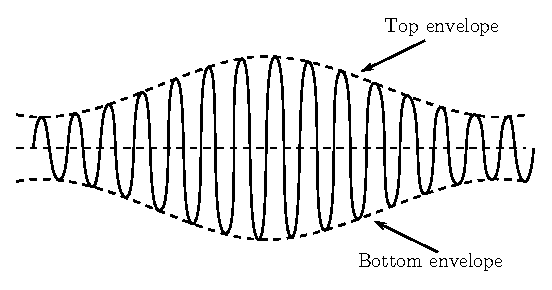
\includegraphics{chap9/fig8.6.eps}
\caption{AM wave}\label{fig9.6}
\end{figure}

Demodulation of AM involves two steps.
\begin{itemize}
\itemsep=0pt
\item Retaining the top envelope by eliminating the bottom envelope. This can be accomplished by a diode which rectifies only one half cycle.

\item Filtering out or removing the high frequency carrier. This can be accomplished by using a parallel RC circuit which is basically a lowpass filter.
\end{itemize}

The AM detector circuit is shown in Fig.~\ref{fig9.7}(a). It contains a diode followed by a parallel RC circuit.
\begin{figure}[H]
\centering
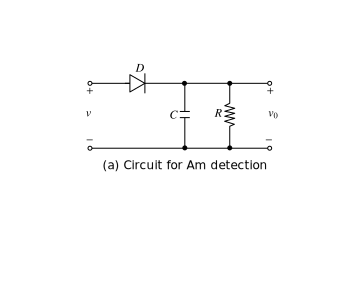
\includegraphics{chap9/fig8.7a.eps}

\medskip
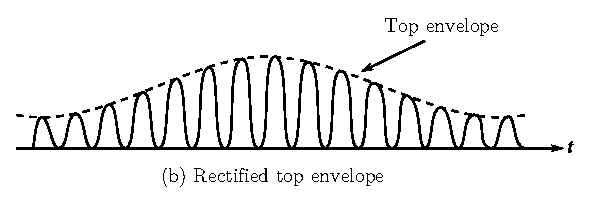
\includegraphics{chap9/fig8.7b.eps}

\medskip
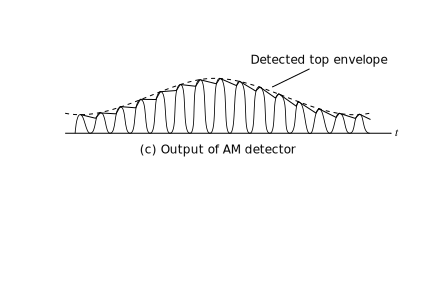
\includegraphics{chap9/fig8.7c.eps}

\smallskip
\caption{Defection of AM}\label{fig9.7}
\end{figure}

The diode rectifies only the top envelope of AM wave as shown in Fig.~\ref{fig9.7}(b). The filtered output is shown in Fig.~\ref{fig9.7}(c). 

To start with, the diode conducts during the rising part of the carrier and charges the capacitor to the peak value of that cycle of the carrier. When the carrier signal begins to fall from its peak, the diode stops conducting and the capacitor discharges into the resistor. The discharging of the capacitor continues until the carrier voltage rises and goes above the capacitor voltage in the next cycle. The diode conducts again and charges the capacitor to the new peak level of the carrier and the same cycle of operations repeat.

Note that the output voltage, $v_{0}$, follows the envelope of the carrier which is nothing but the modulating signal. However there is a small variation in $v_{0}$ due to charging and discharging of $C$. This variation can be minimised by satisfying the following condition.

The time constant RC must be very much greater than the time period, $T_{c}$, of the carrier
\begin{align}
& RC\gg T_{c}\label{eq9.39}\\
& T_{c}=\frac{1}{f_{c}}=\dfrac{2\pi}{\omega_{c}}\label{eq9.40}
\end{align}

Substituting Eqn.~\eqref{eq9.40} in Eqn.~\eqref{eq9.39}, we get
\begin{equation}
RC\gg \dfrac{2\pi}{\omega_{c}}\label{eq9.41}
\end{equation}

If the time constant is too large, the capacitor voltage falls very slowly, the diode may not conduct and charge the capacitor to the next peak. Thus the modulating envelope may not be detected. This situation is avoided by the condition:
\begin{align}
& RC \ll T_{m}\label{eq9.42}\\[3pt]
& T_{m}=\frac{1}{f_{m}}=\frac{2\pi}{\omega_{m}}\label{eq9.43}
\end{align}
where $T_{m}$ is the time period of modulating signal.

Substituting Eqn.~\eqref{eq9.43} in Eqn.~\eqref{eq9.42} we obtain
\begin{equation}
RC\ll \frac{2\pi}{\omega_{m}}\label{eq9.44}
\end{equation}

Combing Eqns.~\eqref{eq9.41} and \eqref{eq9.44} we get
\begin{equation}
\frac{2\pi}{\omega_{c}}\ll RC\ll \frac{2\pi}{\omega_{m}}\label{eq9.45}
\end{equation}

The detected envelope is
\begin{equation}
v_{0}=V_{c}+mV_{c}\sin \omega_{c}t\label{eq9.46}
\end{equation}

The constant term, $V_{c}$, represents dc component which can be easily removed by a lowpass filter.

\section{Angle modulation}\label{sec9.17}
\index{Angle modulation}

In angle modulation the phase or frequency of the carrier wave is varied in accordance with the modulating signal, while the amplitude of the carrier is kept constant. The angle modulated wave is represented by
\begin{equation}
v=V_{c}\cos (\omega_{c}t+\phi(t))\label{eq9.47}
\end{equation}
where the angle $\phi(t)$ is a function of the modulating signal.

\subsection{Two methods of angle modulation}\label{sec9.17.1}
\index{Angle modulation!methods of}

In angle modulation the phase angle of the carrier is varied by two possible methods, namely
\begin{enumerate}
\item Phase modulation (PM).

\item Frequency modulation (FM).
\end{enumerate}

In phase modulation the phase angle of the carrier is varied linearly with the message or information signal $v_{m}$ according to the relation
\begin{equation}
\phi(t)=\omega_{c}t+k_{p}v_{m}\label{eq9.48}
\end{equation}
where, $k_{p}=$ phase sensitivity of the modulator.

The instantaneous value of the phase modulated wave is given by
\begin{equation}
v=V_{c}\cos (\omega_{c}t+k_{p}v_{m})\label{eq9.49}
\end{equation}

In frequency modulation the frequency of the carrier is varied linearly with the message or information signal according to the relation
\begin{equation}
f=f_{c}+k_{f}v_{m}\label{eq9.50}
\end{equation}
where $k_{f}=$ frequency sensitivity of the modulator.

The instantaneous value of frequency modulated wave is given by
\begin{equation}
v=V_{c}\cos \left[\omega_{c}t+2\pi k_{f}\int\limits^{t}_{0}v_{m}dt\right]\label{eq9.51}
\end{equation}

The effect of phase or frequency modulation is that the zero crossing of the modulated wave will not occur at regular intervals.

\subsection{How PM and FM differ from AM?}\label{sec9.17.2}

PM and FM differ from AM in the following ways:
\begin{enumerate}
\item Unlike AM, the zero crossing of PM or FM wave does not occur at regular intervals of time.

\item The envelope of PM and FM waves are constants as compared to that of AM.

\item Unlike AM, the instantaneous value of FM wave is a non-linear function of the information signal. Hence, frequency modulation is a non-linear process.
\end{enumerate}

\section{Frequency modulation}\label{sec9.18}

Frequency modulation\index{Frequency modulation} or FM is a system of modulation in which the frequency of radio frequency carrier is varied in accordance with the instantaneous value of the modulating or information signal, keeping the amplitude of the carrier constant. 

In FM, the information is represented by changes in the carrier frequency. Since the amplitude is constant, noise will not affect the information on the carrier and the power associated with FM wave is constant.


\subsection{Waveforms of frequency modulation}\label{sec9.18.1}

Fig.~\ref{fig9.8} illustrates the principle of frequency modulation. Here the modulating signal and the carrier are assumed to be sinusoidal voltages of amplitudes $V_{m}$ and $V_{c}$ respectively. The angular frequencies of the modulating voltage and the carrier are $\omega_{m}$ and $\omega_{c}$ respectively.

The frequency modulated wave is shown in Fig.~\ref{fig9.8}(c). As shown in Fig.~\ref{fig9.8}(d) the frequency of the carrier changes about its center value $f_{c}$ with variation in the amplitude of the modulating voltage.

When the modulating signal voltage is zero as at points A, C and E in Fig.~\ref{fig9.8}(b), the carrier frequency is unchanged and remains at the center frequency, $f_{c}$ i.e., the frequency of the unmodulated carrier as shown in Fig.~\ref{fig9.8}(c) and (d).

When the modulating voltage approaches its positive peak as at point B, the carrier frequency is increased to a maximum as shown by the closely spaced cycles in Fig.~\ref{fig9.8}(c).

However, during the negative peaks of the modulating voltage as at point D, the carrier frequency is reduced to minimum as shown by the widely spaced cycles in Fig.~\ref{fig9.6}(c).

Thus, the process of FM makes the frequency of the carrier to deviate from its center frequency $f_{c}$ by an amount $\pm \Delta f$, where $\Delta f$ is termed as the frequency deviation. The maximum frequency shift or deviation is denoted by $\delta$.

\subsection{Frequency deviation in frequency modulation}\label{sec9.18.2}

In frequency modulation, the frequency of the carrier is shifted from its unmodulated value by an amount which is proportional to the amplitude of the modulating signal. This shift is termed as {\em deviation} or {\em frequency deviation} and is defined by
\begin{equation}
\Delta_{f}=\frac{\Delta \omega}{2\pi}\label{eq9.52}
\end{equation}
Where, $\Delta\omega$ is the change in the angular frequency of the carrier wave.

The rate at which the carrier frequency changes is equal to the frequency of the modulating signal.
\begin{figure}[H]
\centering
\includegraphics[scale=.95]{chap9/S3-EE-07-007.eps}
\caption{Frequency modulation}\label{fig9.8}
\end{figure}

\subsection{Expression for the maximum frequency deviation of an FM wave}\label{sec9.18.3}

The instantaneous frequency $f$ of the frequency modulated wave is given by
\begin{equation}
f=f_{c}(1+kV_{m}\cos \omega_{m}t)\label{eq9.53}
\end{equation}
where $f_{c}=$ unmodulated or average carrier frequency.
\begin{quote}
$k=$ proportionality constant.

$V_{m}\cos \omega_{m}t=$ instantaneous modulating voltage.
\end{quote}
A cosine modulating voltage is preferred as it simplifies the calculations.

Eqn.~\eqref{eq9.53} can be written as
\begin{equation}
f=f_{c}+\Delta f\label{eq9.54}
\end{equation}
where $\Delta f=kV_{m}f_{c}\cos \omega_{m}t$ is the frequency deviation or shift, which depends on the instantaneous amplitude of the modulating signal, $v_{m}=V_{m}\cos \omega_{m}t$.

The maximum value of $\Delta f$ occurs when $\cos \omega_{m}t$ is maximum which is $\pm 1$. Under such conditions, the instantaneous frequency $f$ will be
\begin{equation}
f=f_{c}(1\pm kV_{m})=f_{c}\pm kV_{m}f_{c}\label{eq9.55}
\end{equation}

Hence, the maximum deviation will be
\begin{equation}
\delta = (\Delta f\,)_{\max}=kV_{m}f_{c}=\frac{kV_{m}\omega_{c}}{2\pi}\label{eq9.56}
\end{equation}
where $\omega_{c}=2\pi f_{c}$ is the angular frequency of the unmodulated carrier.

$k_{f}=kf_{c}$ is called the deviation constant or frequency sensitivity of FM, expressed in kHz\,/\,volt.
\begin{equation}
\therefore\qquad \delta=k_{f}V_{m}\label{eq9.57}
\end{equation}

\subsection{Expression for the FM wave}\label{sec9.18.4}

Let the modulating voltage be
\begin{equation}
v_{m}=V_{m}\cos \omega_{m}t\label{eq9.58}
\end{equation}
and the carrier voltage be
\begin{equation}
v_{c}=V_{c}\sin (\omega_{c}t+\phi)\label{eq9.59}
\end{equation}

Eqn.~\eqref{eq9.59} can be written as
\begin{equation}
v_{c}=V_{c}\sin \theta\label{eq9.60}
\end{equation}
where $\theta=(\omega_{c}t+\phi)$ represents the total phase angle of $v_{c}$ at any instant of time $t$.

The angular frequency $\omega_{c}$ of the carrier can be written as
$$
\omega_{c}=\dfrac{d\theta}{dt}
$$

In frequency modulation the angular frequency of the carrier is varied in accordance with the instantaneous value of the modulating voltage. Hence, the instantaneous angular frequency of the modulated carrier is given by
\begin{equation}
\omega_{i}=\omega_{c}(1+kV_{m}\cos \omega_{m}t)\label{eq9.61}
\end{equation}

But, 
\begin{align*}
\omega_{i} &= \dfrac{d\theta_{i}}{dt} \ \Rightarrow \ \theta_{i}=\int \omega_{i} \,dt\\[3pt]
\text{where},\quad \theta_{i} &= \text{instantaneous phase angle of the modulated carrier}
\end{align*}
\begin{align*}
\therefore\qquad \theta_{i} &= \int \omega_{i}\,dt=\int \omega_{c}(1+kV_{m}\cos \omega_{m}t)\,dt\\[3pt]
&= \omega_{c}t+\frac{kV_{m}\omega_{c}\sin \omega_{m}t}{\omega_{m}}\\[3pt]
&= \omega_{c}t+\frac{kV_{m}f_{c}\sin \omega_{m}t}{f_{m}}\quad [\because \ \omega_{c}=2\pi f_{c}\text{~~ and~~ } \omega_{m}=2\pi f_{m}]
\end{align*}
But from Eqn.~\eqref{eq9.56}, $kV_{m}f_{c}=\delta$ and hence
\begin{equation}
\theta_{i}=\omega_{c}t+\dfrac{\delta}{f_{m}}\sin \omega_{m}t\label{eq9.62}
\end{equation}

The instantaneous amplitude of the frequency modulated or FM signal can be given by
\begin{align}
v &= V_{c}\sin \theta_{i}\notag\\[3pt]
&= V_{c}\sin \left(\omega_{c}t+\dfrac{\delta}{f_{m}}\sin \omega_{m}t\right)\label{eq9.63}
\end{align}

The ratio $\dfrac{\delta}{f_{m}}$ is defined as the modulation index for FM and is denoted by $m_{f}$.
\begin{align}
\therefore\qquad v &= V_{c}\sin (\omega_{c}t+m_{f}\sin \omega_{m}t)\notag\\[3pt]
\text{or}\qquad v &= V_{c}\sin (2\pi f_{c}t+m_{f}\sin 2\pi f_{m}t)
\end{align}
which is the expression for FM wave.

\subsection{Modulation index for FM}\label{sec9.18.5}
\index{Frequency modulation!modulation index}

The modulation index for FM, $m_{f}$, is defined as
\begin{equation}
m_{f}=\frac{\text{maximum frequency deviation}}{\text{modulating frequency}}=\dfrac{\delta}{f_{m}}\label{eq9.65}
\end{equation}

The modulation index $m_{f}$ is generally greater than $1$. Although $m_{f}$ is a ratio of two frequencies, it is measured in radians.

\subsection{Frequency spectrum and bandwidth of an FM wave}\label{sec9.18.6}
\index{Frequency modulation!frequency spectrum}
\index{Frequency modulation!bandwidth of}

Unlike AM, where there are only two sidebands, frequency modulation has infinite number of sidebands, as well as the carrier. The sidebands are separated from the carrier by $f_{m}$, $2f_{m}$, etc.

The modulation index, $m_{f}$ of FM determines the number of sidebands that have significant amplitudes.

Unlike in AM, the carrier amplitude in FM is a constant.

For certain values of modulation index, called eigen values it is possible for the carrier component of FM wave to disappear completely.

Because of the infinite sidebands, the bandwidth of FM is much larger compared to that of AM.

Theoretically FM requires infinite bandwidth. However, in practice the bandwidth used is one that accommodates all those sidebands which have significant amplitudes.

The transmission bandwidth of an FM wave generated by a modulating signal of frequency $f_{m}$ is given by
\begin{align}
\text{BW} &= 2\delta + 2f_{m}\notag\\[3pt]
&= 2m_{f}f_{m}+2f_{m}=2f_{m}(1+m_{f})\label{eq9.66}
\end{align}
This is called Carlson's rule.

\section{FM Detection}\label{sec9.19}
\index{FM Detection}

Phase-locked loop\index{Phase-locked loop} (PLL) is used for the demodulation of\index{Frequency modulation!demodulation of} FM signal. PLL is available in the form of an integrated circuit. NE\,565 is a commercially available PLL\;IC. The block diagram of PLL is shown in Fig.~\ref{fig9.9}.
\begin{figure}[H]
\centering
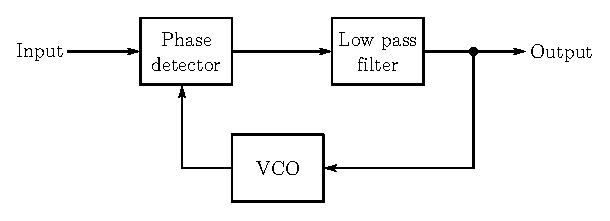
\includegraphics{chap9/fig8.9.eps}
\caption{Block diagram of PLL}\label{fig9.9}
\end{figure}

\eject

PLL consists of the following blocks.
\begin{enumerate}
\item Phase detector (PD)

\item Low pass filter (LPF)

\item Voltage controlled oscillator (VCO)
\end{enumerate}
\begin{itemize}
\item Phase detector produces an output voltage proportional to the phase difference (or frequency difference) between the input and VCO output signals.

\item Low pass filter eliminates high frequency component present in PD output and presents a smooth dc voltage at VCO input.

\item VCO produces an output frequency proportional to the voltage applied at its input, which is nothing but LPF output.
\end{itemize}

\heading{Working}
\begin{itemize}
\itemsep=1pt
\item Under no input signal, the VCO frequency is set at the carrier frequency, $f_{c}$.

\item With FM signal applied:
\begin{itemize}
\item[(i)] If the input signal is unmodulated carrier, input is only the carrier and hence the input frequency is $f_{c}$. PLL output is zero since input frequency and VCO frequency are both $f_{c}$ at the PD input.

\item[(ii)] If the input signal is a modulated carrier, variations are present in input frequency, which is detected by the PD. PLL output voltage changes and causes the VCO frequency to change to match with the FM signal frequency. Thus the PLL output voltage tracks the modulating signal.
\end{itemize}
\end{itemize}

\begin{example}\label{exam9.13}
Given an FM wave $v=10\sin [2\pi \times 10^{8}t+5\sin (2\pi \times 15\times 10^{3}t)]$ find (i) the carrier frequency (ii) the modulation index (iii) modulating frequency and (iv) frequency deviation. What power will this FM wave dissipate in a $10\Omega$ resistor.
\end{example}

\begin{solution}
The FM wave equation is
$$
v=V_{c}\sin [2\pi f_{c}t+m_{f}\sin 2\pi f_{m}t]
$$

The given equation is
$$
v=10\sin [2\pi \times 10^{8}t+5\sin 2\pi \times 15\times 10^{3}t]
$$
on comparison, we get the following
\begin{itemize}
\item[(i)] Carrier frequency, $f_{c}=10^{8}\text{Hz}=100$\.MHz.

\item[(ii)] Modulation index, $m_{f}=5$.

\item[(iii)] modulating frequency $f_{m}=15\times 10^{3}\text{Hz}=15$\,kHz.

\item[(iv)] the frequency deviation
$$
\delta = m_{f}\times f_{m}=5\times 15\,\text{kHz} = 75\text{\,kHz}
$$
The power dissipated in a $10\,\Omega$ resister will be
$$
P=\dfrac{V^{2}_{\text{rms}}}{R}=\dfrac{(V_{c}/\sqrt{2})^{2}}{R}=\dfrac{(10/\sqrt{2})^{2}}{10}=5\,\text{W}
$$
\end{itemize}
\vskip -.7cm
\end{solution}

\begin{example}\label{exam9.14}
A 25\,MHz carrier is frequency modulated by a 400\,Hz audio sine wave. The carrier voltage is $4\text{\,V}$ and the maximum deviation is $10\text{\,kHz}$. Write the equation for this FM wave.
\end{example}

\begin{solution}
Given \ $V_{c}=4\text{V}$, $f_{c}=25\text{\,MHz}$, $f_{m}=400\text{Hz}$~~ and~~ $\delta=10\text{\,kHz}$
\begin{align*}
\omega_{c} &= 2\pi f_{c}=2\pi \times 25\times 10^{6}=157.08\times 10^{6}\text{\,rad/s,}\\[4pt]
\omega_{m} &= 2\pi f_{m}=2\pi \times 400 = 2513.27\text{\,rad/s}\\[4pt]
m_{f} &= \frac{\delta}{f_{m}}=\frac{10\times 10^{3}}{400}=2.5
\end{align*}
the equation of the FM wave is
\begin{align*}
& v = V_{c}\sin (2\pi f_{c}t+m_{f}\sin 2\pi f_{m}t)\\[4pt]
& v = 4\sin [157.08\times 10^{6}t+2.5\sin (2513.27t)]
\end{align*}
\vskip -.7cm
\end{solution}

\begin{example}\label{exam9.13}
In an FM system $k_{f}=1\text{\,kHz}/\text{V}$ and a sinusoidal modulating voltage of amplitude $15\text{\,V}$ and frequency $3\text{\,kHz}$ is applied. Find the maximum frequency deviation and modulation index.
\end{example}

\begin{solution}
Given
$$
k_{f}=1\text{\,kHz\,/\,V}, \ V_{m}=15\text{V}, \ f_{m}=3\text{\,kHz}
$$
maximum frequency deviation is
$$
\delta = k_{f}V_{m}=(1\text{kHz/V})(15\text{V}) = 15\text{\,kHz}
$$
modulation index is
$$
m_{f}=\dfrac{\delta}{f_{m}}=\frac{15\,\text{kHz}}{3\,\text{kHz}}=5
$$
\vskip -.7cm
\end{solution}

\eject

\begin{example}\label{exam9.16}
In an FM system the audio frequency (AF) is $500\,\text{Hz}$, the AF voltage is $2.5\text{V}$ and the deviation is $5\text{\,kHz}$. If the AF voltage is now increased to $7.5\text{V}$, what is the new deviation? If the AF voltage is raised to $10\text{V}$ while AF is dropped to $250\text{Hz}$, what is the deviation? Find the modulation index in each case.
\end{example}

\begin{solution}
\begin{align*}
k_{f} &=\dfrac{\delta}{V_{m}}=\dfrac{5\text{\,kHz}}{2.5\text{V}}\\[4pt]
      &=2\text{\,kHz\,/\,V}
\end{align*}
when $V_{m}=7.5\text{V}$
\begin{align*}
\delta &= k_{f}V_{m}=(2\,\text{kHz\,/\,V})(7.5\,\text{V})\\[4pt]
& = 15\text{\,kHz}
\end{align*}

\vskip .1cm

Similarly, when $V_{m}=10\text{V}$
$$
\delta = (2\,\text{kHz/V})(10\V) = 20 \text{kHz}
$$

\vskip .1cm

Change in modulating frequency does not change deviation as it is independent of modulating frequency.


\vskip .1cm

Calculation of modulation indices:
\begin{align*}
m_{f_{1}} &= \frac{\delta_{1}}{f_{m_{1}}}=\frac{5\times 10^{3}}{500}=10\\[7pt]
m_{f_{2}} &= \frac{\delta_{2}}{f_{m_{2}}}=\frac{15\times 10^{3}}{500}=30\\[7pt]
m_{f_{3}} &= \frac{\delta_{3}}{f_{m_{3}}}=\frac{20\times 10^{3}}{250}=80
\end{align*}
\vskip -.7cm
\end{solution}

\section{Limitations of amplitude modulation}\label{sec9.20}
\index{Amplitude modulation!limitations of}

Amplitude modulation has the following limitations.
\begin{enumerate}
\item {\bf Poor Efficiency:} In AM the useful power is in the sidebands which contains information. However, the power in the sidebands is low and most of the power is in the transmitted carrier which is useless. Thus the transmission efficiency of AM is poor.

\item {\bf Noisy reception:} In an AM wave, the information is represented as amplitude variations of the carrier. Since a radio receiver cannot distinguish between amplitude variations that represent noise and those that represent the desired signal AM reception is generally noisy.

\item {\bf Limited operating range:} Because of poor efficiency transmitters employing amplitude modulation have limited operating range i.e., messages cannot be transmitted over long distances.

\item {\bf Poor audio quality:} The practical limitation on the bandwidth of AM results in interference between adjacent stations leading to poor quality of reception.
\end{enumerate}

\section{Advantages of frequency modulation over amplitude modulation}\label{sec9.21}
\index{Frequency modulation!advantages of}

Frequency modulation has the following advantages over amplitude modulation.
\begin{enumerate}
\item All the transmitted power in FM is useful, whereas in AM most of it is in the transmitted carrier which does not contain any information. So efficiency of FM is high.

\item As FM receivers can be fitted with amplitude limiters to remove the amplitude variations caused by noise, FM reception is more immune to noise than AM reception.

\item In FM there is practically no adjacent channel interference which results in better audio quality than AM reception.

\item FM transmitters operate in the Upper VHF and UHF frequencies at which there is less noise than in the MF and HF ranges used by the AM transmitters.
\end{enumerate}

\section{Disadvantages of FM}\label{sec9.22}
\index{Frequency modulation!disadvantages of}

\begin{enumerate}
\item FM requires wider channel or bandwidth, upto 10 times more than that needed by AM.

\item In FM, the area of reception is small as it is limited to line of sight.

\item FM requires complex and expensive transmitting and receiving equipment.
\end{enumerate}

\eject

\section{Comparison between AM and FM}\label{sec9.23}
\index{Modulation!comparison between}

Table~\ref{tab9.2} gives a comparison of AM and FM, highlighting their relative merits and demerits.
{\renewcommand{\arraystretch}{1.2}
\begin{longtable}[c]{|r|p{5.7cm}|p{5.7cm}|}
\caption{Comparison between AM and FM}\label{tab9.2}\\
\hline
Sl. No. & \multicolumn{1}{c|}{\bf Amplitude Modulation} & \multicolumn{1}{c|}{\bf Frequency Modulation}\\[3pt] 
\hline
1.~~~ & In AM, amplitude of the carrier varies while its frequency remains constant & In FM, the frequency of the carrier changes while its amplitude remains constant\\
\hline
2.~~~ & Modulation index $(m_{a})$ can have values from 0 to 1 only & Modulation index $(m_{f})$ is much greater than 1\\
\hline
3.~~~ & AM has only two sidebands & FM has infinite number of sidebands\\
\hline
4.~~~ & The bandwidth is twice the highest modulating frequency : $BW=2f_{m}$ & Bandwidth is much larger than AM : $BW=2(\delta+f_{m})$\\
\hline
5.~~~ & Carrier frequency is in the lower RF-500 kHz to 3 MHz &  Carrier frequency is very high - VHF and UHF (88 to 108 MHz)\\
\hline
6.~~~ & Susceptible to noise & More immune to noise\\
\hline
7.~~~ & Propagation is by ground waves and sky waves & Propagation is by space waves\\
\hline
8.~~~ & AM transmission covers long distances & FM transmission covers smaller distances only (line of sight)\\
\hline
9.~~~ & Requires less complex and less expensive equipment & Requires more complex and expensive equipment\\
\hline
10.~~~ & AM has less transmission efficiency & FM has better efficiency but not better than AM with suppressed carrier\\
\hline
11.~~~ & Distortion occurs in AM due to common channel interference (CCI) & Distortion due to CCI is less in FM.\\
\hline
\end{longtable}}\relax

\newpage

\begin{center}
\rule{5cm}{1pt}\\[-2pt]
{\bf Exercise Problems}\\[-4pt]
\rule{5cm}{1pt}
\end{center}
\begin{enumerate}
\renewcommand{\labelenumi}{\bf\theenumi.}
\item A \ 1\,kW \ carrier is modulated to a depth of 80\%. Calculate the total power in the modulated wave.

\item The total power content of an AM wave is 4\,kW at a modulation factor of 80\%. Calculate
\begin{itemize}
\item[(a)] Carrier power

\item[(b)] Power in each sideband.
\end{itemize}

\item An AM broadcasting station broadcasts with an average transmitted power of 30\,kW at a modulation index of 0.8. Find
\begin{itemize}
\item[(a)] The transmission efficiency

\item[(b)] Power in the carrier.
\end{itemize}

\item An AM broadcasting station broadcasts with an average transmitted power of 25\,kW. The modulation index is set at 0.75. Find the saving in power if the power contained in the LSB alone is used.

\item A 40\,MHz carrier is frequency modulated by a 500\,Hz audio sine wave. The carrier voltage is 5\,V and the maximum deviation is 10\,kHz. Write the equation for this FM wave.

\item In an FM system $K_{f}=1\,\text{KHz/V}$ and a sinusoidal modulating voltage of amplitude 12\,V and frequency 4\,kHz is applied. Find the maximum frequency deviation and modulation index.
\end{enumerate}
